\section{Data Analysis and Results}
In the following section, the hand-washing trials, the SRS survey, entrance survey, and post-interventions survey, and the parent interviews are analyzed qualitatively, and the annotated video data of the hand-washing trials is analyzed quantitatively.  

\subsection{Participants Recruited}
Due to limitation of time, we were only able to recruit one subject.  Our participant is a thirteen years old male child of Asian ethnicity.  He was accompanied to the trials by his mother, who was the one that answered all surveys.

\subsubsection{Entrance and SRS Survey Results}
The following backgrounds of the child were reported by the entrance and SRS surveys.  The purpose of this section is to familiarize the reader with our participant and understand better the context that our study results situate in.

\paragraph{Child's Demographics and Inclusion Criteria Fit}
The parent reported that the child has been clinically diagnosed of Autism Spectrum Disorder.  We also conducted the Social Responsiveness Scale Survey, and the child obtained a T-score of 79, passing the minimum score for severe ASD.  Through the Entrance Survey, we learned that the child has difficulty independently completing self-care activities (a 2 on a scale of 1 (not independent at all) to 5 (completely independent)), and this includes hand-washing (also a 2 on the same scale).  We also learned that the child is able to but not good at verbal communication (a 3 on a scale of 1 (very not well) to 5 (very well)).  Specifically, the child can only speak one or two words at a time to express what he wants, uses iPad for communication, and often just murmurs illegibly.  However, the child has the ability to follow simple, one-step verbal instructions (a 4 on a scale of 1 (very not well) to 5 (very well)).  Lastly, the child does not exhibit severely aggressive behavior (a 1 from a scale of 1 (never) to 5 (often)).  The above shows that the child fits our inclusion criteria.

\paragraph{Child's Experience with Technologies}
The childf is more of a visual learner.  He uses a computer at home, and likes to use it very much.  He also likes to use other technologies (e.g. iPhone, iPad), and likes to watch movies and TV.  He doesn't have a robot toy to play with at home or at school, so the parent doesn't know how much he likes to play with robot toys.  The parent never used technologies to help the child with self-care activities except using pictures to teach step by step hand-washing.

\paragraph{Child's Personal Preferences}
The child is sensitive to sound.  He likes Disney cartoon musics, and likes to watch his favorite cartoon scenes repeatedly on the iPad.  To reward the child after a good behavior, the parent suggested the following rewards: give extra time to play on iPad, give him praises (e.g. good job), give children books to read and animal dinosaurs to play with, give the parent's iPhone since the child's favorite musics are on there.

\paragraph{Child's Abilities on Hand-washing and on Other ADLs}
The parent agrees that the child usually gets distracted when performing hand-washing.  To assist him, the parent mainly reminds him to put soap, rinse properly, and dry properly with towel.  He needs more prompting in these areas since he always washes in a hurry.

Other activities the child needs help with include:  tooth brushing -- 2 hours/week; bathing -- 4.5 hours/week; dressing -- usually just hand the clothes to him, he knows how to put them on, but needs reminders of the order of the clothing, 7 hours/week.

\paragraph{Parent's Expectation and Concerns}
The parent expected the robot to be helpful in reminding the child to put soap, rinse and dry more, similar to the role of M.  Some concerns the parent has include: the child may be wondering why does he need to wash hands so many times repeatedly; the child performs well in his comfort zone with the same environment, so it takes a while for the child to get used to the lab environment.

\subsection{Case Selected}
Our participant fits the inclusion criteria as a user with typical use case for the robot.  It was noted that the typical use cases for the robot may be several, depending on the kinds of helps the user needs.  From the background report above, we understood that the child mainly needs help initiating the hand-washing activity, and guidances during certain steps (i.e. the get soap, rinse, and dry steps), but the child does not need much prompts for demonstrating the actions of each step.  This tendency of the child was verified during the trials, and we attempted to answer the question how ``best to prompt the child'' given this tendency (e.g. Should we prompt only the steps the child needs help, or prompt every step to create consistency?  Should we still demonstrate actions for the prompted steps or skip the MoDemo part of the prompt entirely?)  These will be answered in our discussions.

\subsection{Qualitative Data Analysis Method}
The sources of data collected for qualitative data analysis included child hand-washing trials videos, between trials parent researcher interview transcriptions, and after trial parent survey.  With these data, as well as researcher's self reflections, we would attempt to answer what are the parent's and researcher's thoughts on how did the child receive the robot as a prompting agent and how to improve the robot, the prompting protocol, and the research study.

The child hand-washing trials videos were only used as a reference to go back to if uncertainties arose in analysis that needed verifications.  They were not used as a primary source of data to generate themes.  Instead, the process of making field notes based on observations of the child's behaviors during the hand-washing trials were achieved by the parent researcher discussion interviews during the breaks between trials.  Then, the transcriptions of parent researcher interviews were analyzed from trial to trial, and the ``constant comparative method'' was applied to distill common categories or themes that cut across all trials.  In concise words, the ``constant comparative method'', as described by Merriam, is an analysis method commonly used in qualitative researches that involves comparing ``one unit of information with the next in looking for recurring regularities in the data'' \cite{merriam2014qualitative}.  Categories are formed that the data relevant to the research questions fit into.  And as we go through more units of information, these categories may be subdivided or subsumed under more abstract categories as we ``begin to discriminate more clearly between the criteria for allocating data to one category or another''.  As a side note, this process focuses on describing the data in a concise and logical way rather than on evaluating hypotheses.

Lastly, themes distilled from the parent's post intervention survey were reported on improving robot, prompting protocol, and research study.  In addition, the researcher would self reflect on these topics and give inputs as the person who operated the robot and conducted the study.

%this is the qualitative data results section
\subsection{Qualitative Data Analysis Results}
In this section, qualitative data analysis results are reported.  We first compare and contrast between parent prompting and robot prompting on how the prompts were delivered and how well did the child receive them.  Then we examine the factors contributing to the child's difference of reception of robot prompts and the parent prompts.  Lastly, we explore changes to the robot and the study that did or would possibly improve robot prompt reception from the child.

\subsubsection{Parent Prompts - Phase A}
During Phase A, where the parent alone prompted the child through hand-washing steps, the parent was not instructed on what or how to prompt by the researcher.  The only input given to the parent during this phase was to get the child to rinse more and dry more.  The parent had no prior knowledge of how the robot prompts were going to be like either.  Thus, the way the parent prompted was very similar to how she'd have prompted at home in everyday settings, and one she probably found effective to her son.

The sequence of hand-washing steps the parent prompted was in the following order: get soap, lather, turn on water, rinse, turn off water, dry.  This order is one of the many logical orders of hand washing, since one could alternatively choose to turn on water before lather so one could lather in the running water, or even to turn on water before getting soap, so one's hand is wet when lathering.  However, the parent chose to get soap and lather first before turning on water, probably because of her and the child's habits, and she had not changed this sequence order through out the trials in Phase A.  Although, an interesting thing to note is, whenever the parent did not prompt for lather right after get soap and leave the child to decide which steps to do, the child would always turn on the water first after getting soap and lather in water.

The parent used verbal prompts as the major prompting modality, although for some steps, she also prompted using gestures such as pointing and motion demonstration.  The parent's prompting patterns most common for each step are summarized in Table \ref{tab:ParentPrompts}.  In the table, ``MoDemo'' refers to motion demonstration gestures (e.g. rubbing hands together for lather step and flipping and turning hands in the air for dry step).  ``Point'' refers to pointing to the object of interaction (e.g. the water during rinse step).

\begin{table}[H]
	\centering
	\begin{tabular}{ | l | l | l | }
		\hline
		\textbf{Step}	&	\textbf{Verbal Prompt} & \textbf{Gesture Prompt}	\\	\hline	\hline
		
		Get soap	&	Get some soap; Soap;	&	- 	\\	\hline
		Stop soap	&	Just one; That's it; Enough; That's too much;	&	-	\\ \hline
		Lather	&	Lather your hands; Lather; Soap;	& MoDemo	\\	\hline
		Turn on water	&	Turn on the water;	&	-	\\	\hline
		Rinse	&	Rinse more; Water; More water; Wash hands; More;	&	MoDemo; Point	\\	\hline
		Turn off water	&	Turn off the water;	&	-	\\	\hline
		Dry	&	Dry; More Dry; Towel; Dry your hands; More;	&	MoDemo	\\	\hline
		
	\end{tabular}
	\caption{Parent Prompts}
	\label{tab:ParentPrompts}
\end{table}

For the lather, rinse, and dry steps, they are not single action steps, but need continuous motions.  For these steps, the parent would repeatedly deliver verbal prompts of the same step every two seconds or so, until the parent was satisfied with the step's duration.  Variations of the step's verbal prompt were often used (e.g. shortening ``dry your hands'' to ``dry'', or add the word ``more'' or simply using ``more'' for verbal prompts).  The variations can be seen in Table \ref{tab:ParentPrompts}.  Most often for the lather step, and sometimes for the rinse and dry steps, the parent also delivered continuous motion demonstration, and would verbally prompt ``like this'' for the child to follow.  Note that the parent used ``soap'' for verbal prompt of both get soap step and lather step, but the child understood what to do since the parent always delivered motion demonstrations for the lather step.

The timing of prompt deliveries can be categorized as the following:
\begin{itemize}
	\item \textbf{Proactive Prompt}: prompting a new step before the child finishes current step
	\item \textbf{Corrective Prompt}: prompting the same step when the child is doing or is attempting to do a wrong step
	\item \textbf{Reactive Prompt}: prompting when the child is waiting for prompts
	\item \textbf{No Prompt}: letting the child do what he wants without objections
\end{itemize}
The parent delivered proactive prompts most of the times, prompting the next step right when or before the child finished the current step.  However, sometimes corrective prompts were needed when the child was not complying or executing correctly.  There were also a few times that reactive prompts were needed, for example during rinsing, when the child terminated the step early but was waiting for the parent's permission to go on to the next step.  The parent either told the child to keep doing the current step or acknowledged that the child can proceed to the next step.  The last and the least common scenario was the parent delivering no prompts.  This happened when the parent waited to see if the child knew what to do without being prompted, and the child either executed the correct step for the appropriate duration, needing no prompts, or executed incorrectly or for too short or too long of a duration, but the parent let it go without correction.

In addition to the step prompts, the parent also delivered verbal rewards, but usually only at the very end of each hand-washing trial when the child is all done, saying ``good job''.  Also, during the hand-washing, the parent's gaze was mainly focusing on the object being prompted, and very little eye contacts between the parent and the child were seen.  However, during the verbal reward after the child is all done, the parent would often initiate eye contacts.

The child was generally good in complying to the parent's prompts, although at times noncompliance still occurred.  Systematically, the child's compliance can be categorized into the following four scenarios:
\begin{enumerate}
	\item Waiting to be prompted before executing a step
	\item Executing a step as prompted
	\item Keep executing a step until prompted otherwise or verbally awarded
	\item Terminating a step after being prompted for another step
\end{enumerate}
And conversely, noncompliance are any scenarios outside of the compliance scenarios.  The five common noncompliance scenarios the exhibited include:
\label{List:NoncopmlianceBehaviors}
\begin{enumerate}
	\item Executing a step before prompted
	\item Executing the wrong step after prompted
	\item Idling after prompted
	\item Terminating a correct step before prompted for another step or verbally awarded
	\item Not terminating a correct step after prompted for another step
\end{enumerate}

Specifically, the child was able to wash hands well under the parent's prompting.  The child would usually start the get soap step first, and he'd start the step by himself if the parent did not proactively prompt it.  There were times, however, when the child pressed the soap sprout too many times, and the parent had to prompt him multiple times for him to stop.  The lather step was prompted proactively by the parent with MoDemo gestures, and the child followed it obediently for the whole duration, without terminating the step by himself.  The turn on water step is easy for the child, he'd do it by himself right after the get soap step and lather in water if the parent didn't prompt proactively, or he'd execute the lathering step first if the parent prompted proactively for lathering.  The child would always immediately start rinsing (or lathering in water) by himself after turning on water, without waiting for the rinse prompt.  He could execute the motion of this step well, but the challenge was for him to rinse longer.  After about eight seconds of rinsing in water, he'd terminate the step by himself, and wait for the parent to prompt the next step.  If the parent continued to prompt for the same step (i.e. rinse more), he'd put his hands in the water for one second and withdrew it and wait for the next prompt.  However, he would not start the turn off water step by himself without getting prompted or approval from the parent.  When the parent prompted for turn off the water, the child had no problem following the prompt and executing it.  In addition, he would always start the drying step by himself immediately after turning off the water.  The drying step was a little challenging for the child in both its motion and duration.  The child's motion was mostly drying the inside of his hands, without turning the towel or hand to dry the outside.  However, the parent only demonstrated the motions occasionally, and the child did not change his drying actions even after observing the MoDemo prompts.  The duration of the drying step was around eight seconds before the child decided to terminate the step by himself.  The parent only proactively prompted to dry more while the child was drying, but did not prompt to object when the child decided to terminate the step by putting down the towel.  The parent instead would nod and approve the child to leave the sink once he put down the towel.

The one step the child was openly not complying to the parent's prompt is to terminate the get soap step, where the parent verbally prompted the child to stop many times, but the child still kept pumping the soap onto his hands.  Also, sometimes the child did not want to rinse for the full duration despite the parent prompting rinse more.  The strategies the parent used in dealing with these noncompliance behaviors were:
\begin{itemize}
	\item Proactively prompting before the child executes wrongly
	\item Repeatedly prompting with no pause
	\item Mention the child's name in the verbal prompt
	\item Shortening the verbal prompt into a one or two word phrase and increase in severity of tone when repeating the prompt
	\item Demonstrating the motion with fast moving and continuous gesture prompt
	\item Physically intervene by guiding the child's hands in executing the correct actions
\end{itemize}
The first five strategies were mostly working, and only rarely did the parent need to physically intervene (only for stopping the get soap step).

In addition, sometimes the child played with the soap bubbles in the sink during hand-washing.  The parent prompted ``no playing with the bubbles'', and the child would usually comply.  There was once, though, when the child played with the soap bubbles after rinsing, and the parent prompted for him to rinse again.  However, the child was confused in or did not want to comply to what the parent wanted, and started washing hands from the get soap step once more.

The child seemed to experience fatigue after few trials into each visit, although we had breaks between each trial for around three minutes each.  The fatigue behaviors included playing with bubbles, getting too much soap, terminating rinse steps early, and rushing through the dry steps.  These behaviors were found more likely to occur by the later trials of each visit.

Lastly, the child had a tendency to repeat the verbal prompts after hearing it.  The words he said were not very clear, it's almost like a murmur, but his parent confirmed he was repeating the verbal prompts in order to process it.

\subsubsection{Robot Prompts - First Phase B}
The robot prompting trials spanned three phases, namely and in the order of: the first Phase B, Phase C, and the second Phase B.  The robot prompting protocols were described in Section \ref{sec:SpecificProtocol}.  However, improvisations from the operator as well as changes to the robot behavior and study protocol were needed as the study progressed.

In the first Phase B, the robot was introduced to the child for the first time, and it prompted alone in the washroom.  The operator tried his best to prompt for all seven steps (i.e. turn on water, wet hands, get soap, scrub, rinse, turn off water, dry).  However, due to unfamiliarity with and the lack of ease of the robot control interface and unfamiliarity with the child's behaviors, the operator could not control the robot to keep up with the child's pace.  There were often four to eight seconds of pauses between each new robot prompts, and one to two seconds of pauses between repeats of the same prompt.  In addition, due to the way the robot gestures were implemented, each robot prompt was around four seconds to execute.  Thus, it's possible for the child to execute several steps on his own before the robot prompted another step.  And this was often the case for short steps (e.g. turn off water), requiring the operator to plan and predict the child's behavior ahead of time in order to make the robot prompts relevant and up to the child's current progress in the hand-washing activity.  It also required the operator to refrain from prompting all seven steps, but to only choose three or four important steps to prompt.

The operator was able to focus on delivering the prompts for turn on water, get soap, and rinse steps.  The operator experimented with prompting turn on water as the first step versus prompting get soap as first step.  However, the child was determined to get soap first, despite the robot's repeated first prompts of turn on water.  In one trial, the parent intervened verbally, but it was not until three repeated verbal prompts from the parent that the child complied to turn on water instead of getting soap.  And the compliance did not persist, the trial after that, the child immediately reverted back to getting soap first regardless of robot prompts when the parent is not present.  One thing to note, however, is for the trials that the robot did prompt get soap as first step, the child would not respond immediately or would start the step before waiting to be prompted.

In addition, the operator was not able to prompt the wet hands or scrub steps because the child would start rinse step immediately following turning on water step by himself.  For rinse step, due to robot delay, there are usually four to eight seconds between the previous prompt and the rinse prompt (the longer eight seconds pause happened when the robot gave verbal reward for the previous step, which took three seconds or so itself).  The child had finished rinsing during this delay (the child usually rinsed four seconds before stopping in these first Phase B trials), and would just wait for the robot to prompt.  However, upon hearing the robot prompting the rinse step, the child would take it as a cue to turn off water and start the dry hands step instead of rinse more.  This had been the case for all trials in the first Phase B, and the child's behavior would not change even when the robot repeatedly prompted the rinse step nor when the parent came in to verbally intervene.  The child may be misunderstanding the robot's rinse prompt, or may be simply disobeying its prompts.  But as a consequence, the child finished hand washing before the robot could prompt any more steps after rinse, and thus the robot did not have a chance to prompt the turn off water or the dry hands steps.

The first step was prompted proactively, but most of the other steps were prompted reactively or correctively due to delays in the robot prompt deliveries.  There were also many no prompts, as the operator was prioritizing on prompting only key steps due to robot prompt delays.  The child's compliance to the robot prompts were minimal to nonexistent.  Though the child appeared to be waiting for the robot prompts in the very first couple of trials, the child quickly lost interest in doing so because of the lack of responsiveness of the robot.  Instead, the child mostly ignored the robot and washed hands on his own for the later trials.  The child's noncompliance behaviors were found in all five scenarios listed previously in the parent prompt section \ref{List:NoncopmlianceBehaviors}.

The robot's strategies to deal with noncompliance from the child included repeating the prompt again and the use of attention grabber (AG) by calling the child's name.  Repeating the prompt did not work.  AG did not work either, the child never looked over at the robot because of AG.  Sometimes, noncompliance continued even with the parent coming in and verbally prompting as well.

The child's gaze was on the robot more in the first couple of trials, but in later trials the child did not look at the robot much.  This gaze behavior of the child seemed to correlate with whether he was waiting for the robot.  In light of this, it might be the case that the gaze behavior of the child on a prompting agent is an indication of the child's level of interest, which correlates to the child's willingness to wait for the agent's prompts.

Verbal rewards were used more often in the first few trials.  However, because it delayed the delivery of the proceeding prompt, the operator decided to decrease the frequency of verbally rewarding the child in the later trials.  This did not seem to have a negative effect on the child's level of engagement, it only made the robot prompt deliveries more immediate.

\subsubsection{Robot Prompts - Phase C}
In the Phase C trials, we implemented some changes to how the robot prompted as well as the parent's involvement in hope to improve the child's compliance to robot prompts.

For robot prompt changes, we mainly focused on improving the prompt delays by decreasing the pause between prompts through speeding the gesture animations and eliminating blank periods in the animations.  In addition, the robot control interface was changed from touchscreen input to keyboard input, and a queue was implemented in the robot control scheme so that a sequence of gestures can be requested together at a time, ensuring minimal pause between prompts.  Lastly, after the first Phase B trials, the robot operator also improved in his familiarities with the robot controls as well as to the child's behavior patterns.  These changes resulted in smoother and more responsive robot behaviors in Phase C compared to the first Phase B trials.

The parent took a much more active role in Phase C.  Her involvement can be categorized into three modes.  The first mode attempted was using verbal and gesture prompts very similar to how the parent prompted back in Phase A.  However, the parent quickly realized that prompting in this manner in competition with the robot's prompts appeared confusing to the child, as the child might be overloaded with multiple sources of verbal instructions and gestures, not knowing which source to focus on or obey, decreasing the prompts' effectiveness.  As a result, the parent switched to the second mode of involvement, where the parent only prompted using pointing gestures, and sometimes motion demonstrations, and refrained from any verbal prompts besides telling the child to listen to the robot.  Also, the parent would prompt right after the robot prompted, enforcing the robot instead of competing against it.  Although the parent remained in this mode of involvement for most of the Phase C trials, she also used a third mode of involvement once in a while, to further deepen the pattern of complying to the robot in the child.  This third mode of involvement consists of the parent standing behind the child, and physically guide the child through the steps as the robot prompted, showing the child what an ideal hand-washing trial should look like (it involved waiting for the robot's prompt, obeying the robot, and persisting in a step until otherwise prompted).  In addition, the parent did not remain fully guiding the child's arms for all trials of the third mode.  For later trials of this mode, the parent reduced the intervention level by only nudging the child's elbow as cue to follow the robot, refrained from nudging if the child seemed to perform correctly, and resorted to full guidance of arm if the child was not performing correctly.

The Phase C trials can be viewed as a training phase to teach the child to comply to the robot.  The child seemed to improve in his compliance to robot prompts during Phase C.  The child's improvement can be seen in the following ways:  Firstly, right after getting soap, the child used to immediately turn on water by himself.  However, starting at the second half of Phase C (there was a week between first half and second half of Phase C), the child started to wait for the robot's turn on water prompt before turning on the water.  Secondly, the child used to only follow rinse prompts from the parent, but not the robot.  However, starting at the second half of Phase C, the child begun to follow the rinse prompts from the robot as well.  In addition, the child used to terminate the rinse steps on his own, but starting at second half of Phase C, the child showed longer rinse durations without self termination of the rinse step, sometimes rinsing the full duration marked by the robot delivering a verbal reward or prompting for the turn off water step.  Next, the child used to turn off the water on his own and move on to the dry hands step immediately after terminating the rinse step, but we saw improvements in Phase C of the child waiting more often for the robot's turn off water prompts before executing.  Lastly, however, the dry hands step had very little improvements.


\subsubsection{Robot Prompts - Second Phase B}
In the second Phase B, we resumed back to the robot prompting the child alone, and the parent had minimal involvement.  This phase was used to see if the improvements observed in the training trials of Phase C persisted.  One thing to note is, this phase happened three weeks after the start of Phase C, thus further improvements over the second half of Phase C were not surprising.

First off, after getting soap, the child's improvement in waiting for turn on water prompt from the robot before executing persisted.  In addition, during the soap step, the child begun to listen to the robot's prompt of terminating getting soap and moving on to the turn on water step.  This behavior was only seen rarely at the end of Phase C, but was more prominently observed in the second Phase B.  Next, rinsing after robot's prompts were retained consistently, as well as not terminating the rinse step by himself.  However, in times that the child did terminate the rinse step, he'd still move on to turning off the water without waiting to be prompted.  Lastly, still no improvements on the dry step were observed.

\subsubsection{Causes of Child's Non-Compliances}
Between trials, the researcher (also taking the role of the robot operator) had frequent interview discussions with the mother (referred to as ``the parent'' in above analyses), and occasionally with the father, regarding reasons why the child had problems following the robot.

One major problem pointed out by both of the parents as well as the operator was the delay between each robot prompts.  This problem was particularly significant for our participant, who knew most of the steps of hand-washing, and only needed robot prompts to get started, to terminate the soap step, to rinse more, and to dry more.  Because of his familiarity with the hand-washing steps, he finished each step very quickly and was eager to move to the next step.  Thus a slight delay from the robot would result in the child not waiting for the robot prompts and proceeding on his own.  The mother first pointed this out in the first Phase B, and the operator echoed her opinion, reflecting that it is hard to make the robot keep up with the child due to his pace and the robot delay.  The father also confirmed the opinion in the second Phase B that there should be less pause between prompts, especially for the rinse more prompts, as to prevent the child from moving onto the next step on his own.  Note that the father's opinion was based on the robot behavior after its improvements made to shorten its delays.

In addition, the parents proposed that unfamiliarity was a major cause of the child was not following the robot prompts.  One possible cause for the child's noncompliance was his unfamiliarity with the robot and the washroom environment.  Both parents suggested that the child would be more relaxed and likely not rush each step if he was in a familiar environment, such as at home.  Furthermore, compliance would be greatly improved if the child and the robot built a relationship over time, the mother suggested, and if the robot was always there telling the child what to do, said the father.  To expend on his point, the father explained that the robot needed not to be an authoritative figure like his parents, but just needed to be a figure that the child is familiar in following instructions from, as exemplified by the child's tendency in following his younger brother's instructions.  The father further claimed that it's familiarity and routine, not trust.  The researcher noted that the environmental conditions between the parent trials and the robot trials were similar.  Thus, although being familiar with the environment would possibly improve compliance, the factor that contributed to the difference of child's compliance to the robot and to the parent can only be attributed to his unfamiliarity with the robot, not the environment.

Another possible cause for the child's noncompliance was fatigue due to repetitive consecutive hand-washing trials.  As pointed out by the father, during the robot trials, the child has been asked to wash his hands ten times in a roll with only five minutes of break between each time.  In addition, the robot prompted the rinse step for more than fifteen seconds each time, both of these may make the child unwilling to follow.  The father suggested to conduct each trial two to three hours apart, and prompt rinsing for only ten to fifteen seconds each time.  After further investigation, the researcher noted that the child's fatigue behavior was not specific to the robot, but also present during Phase A when the parent alone prompted the child.  The behavior manifested in the form of the child not willing to rinse more, but the exhibition of it was more subtle in the parent prompting case -- the child would comply to the parent's rinse more prompts, but he would only put his hands into the water for one second and quickly withdrew them and turned to look at the parent for approval to proceed to the next step, where as the child would openly refuse to rinse more in the robot's case.

Another possible cause for noncompliance was the child being confused of what was prompted or what was expected of him by the prompt.  However, there were evidences that the child understood most of the robot verbal prompts, if not all, because he was able to follow them at some point or another.  Thus, for the steps that the child did not follow, one can argue that it must have been due to a cause other than being generally confused of what's prompted.  The mother also confirmed that she thought the child was not confused by the robot prompts.  There were occasions when the child was confused, and they were when the parent pointed to the towel for the child to dry more after the child decided to leave the washroom.  The child would often mistook the parent's pointing gesture for rinse more, and started rinsing again instead of drying.  No such behavior occurred for robot prompts.


\subsubsection{Causes of Improvements of Child's Compliance}
There are three major factors identified by the researcher in potentially causing the improvements observed in the child's compliance to robot prompts: the first one was the improvements made to reduce robot prompt delays; the second was the child's gradual adjusting to the robot and to the routine of following its prompts; and the third was the effect of the trials in Phase C when the parent trained the child to follow the robot prompts.  Of course, there might be other important factors that happened during the time the child spent outside of the lab that were unaccounted for.

In regards to these three factors, the robot prompt delay improvements were seen as the least significant, since after the improvement, we still could not achieve the responsiveness that the parent had during prompting.  The father also expressed he was not satisfied with the improved robot's responsiveness.   In addition, the effect on child's compliance by increasing the robot's responsiveness to the level of the parent was still unknown.  As to the other two factors, both involve the child learning to be guided by the robot, one from natural familiarization by himself and the other due to artificial training from the parent.  One may argue that, since the improvements mostly occurred after the second half of Phase C, it may suggest that the effect of artificial training from the parent is more dominant, since if it were the other way, then the child would have shown improvements earlier (e.g. after the first Phase B or during first half of Phase C).  However, this claim still lacks concrete evidence, and this question should be answered more rigorously by introducing a longer first Phase B that is comparable to Phase C (in our study, we had one week for first Phase B, but two weeks for Phase C) so that the learning effects of the two phases can be compared.


\subsubsection{Post-Intervention Survey for Parent}
The post-intervention survey results are presented in Table \ref{tab:PostInterventionSurveyData}.  We see that the parent was happy with all aspects of the robot as a prompting agent, but did not see it to be as good as herself yet.  The suggestions the parent made regarding the robot and the experiment are reported in the discussion section.

\begin{table}[H]
	\centering
	\begin{tabular}{ | p{12cm} | l | }
		\hline
		\textbf{Survey Question}	&	\textbf{Parent's Answer}	\\	\hline	\hline		
		Hand-washing steps break down was appropriate	&	Strongly Agree	\\	\hline
		My child understood the verbal prompts	&	Agree	\\	\hline
		Robot's verbal prompts were appropriate	&	Strongly Agree	\\	\hline
		The prompt wordings were similar to mine	&	Strongly Agree	\\	\hline
		The prompt voice and tone were appropriate	&	Strongly Agree	\\	\hline
		The prompt wordings were easy to understand	&	Strongly Agree \\	\hline
		My child understood the gesture prompts	&	Strongly Agree	\\	\hline
		The gesture prompts were appropriate	&	Strongly Agree	\\	\hline
		The gesture prompts were easy to understand	&	Agree	\\	\hline
		The physical appearance of robot is aesthetically pleasing	&	Agree	\\	\hline
		The attention grabber gestures were appropriate	&	Strongly Agree	\\	\hline
		The verbal rewards were appropriate	&	Strongly Agree	\\	\hline
		The reward gestures were appropriate	&	Strongly Agree	\\	\hline
		The robot was effective in assisting my child through hand-washing	&	Strongly Agree	\\	\hline
		The robot motivated my child to wash hands	&	Strongly Agree	\\	\hline
		The robot was fun for my child to use	&	Strongly Agree	\\	\hline
		My child was confused by the robot	&	Disagree	\\	\hline
		I like the idea of a robot prompting my child	&	Strongly Agree	\\	\hline
		The robot is able to provide guidance as well as I can or better	&	Neither Agree or Disagree	\\	\hline
		I would want to own a robot like this one	&	Strongly Agree	\\	\hline
	\end{tabular}
	\caption{The Post-Intervention Survey Data}
	\label{tab:PostInterventionSurveyData}
\end{table}


%rename this section to simply report sample selection
%when should i discuss parent's decision on how to involve during phase C?  should have been in the qualitative results section
\subsection{Experiment Design Change}
We were not able to counterbalance the confounding effect of learning through randomly assigning participants to phase orders (A-B-C versus A-C-B), since we only recruited one participant.  Instead, we decided to control it by splitting the Phase B into two segments, one before Phase the child and one after.  Thus, we conducted the study in the following phase order: A-B-C-B (i.e. parent alone phase - robot alone phase - robot parent phase - 2nd robot alone phase).  This way, we can compare first Phase B and second Phase B to see how much does learning in Phase the child affect our results.  Also, first Phase B and second Phase B won't have sixteen trials each due to limitation of time.  Instead, we conducted these two phases only long enough to see a stable response, as is typically done in a single-subject research design \cite{ayres2009acquisition, bereznak2012video}.  As a result, we had 16 trials for Phase A, 8 trials for first Phase B, 21 trials for Phase C, and 5 trials for second Phase B.  Note that the intervention conditions of first Phase B and second Phase B are meant to be the same.


\subsection{Video Data Analysis and Results}
\label{sec:VideoDataAnalysisAndResults}

\subsubsection{Analysis Method}
The analyses employed here are visual analyses.  The analyses mainly compare the levels (eyeballing the mean) of measures in different phases.  In cases where the level of a measure changes dramatically within a phase, this trend with initial level and final level were noted.

\subsubsection{Prompt Effectiveness}
To reflect how effective our prompting system is, we show whether the system can reduce both the number of incomplete steps and the number of parent prompts.

\paragraph{Number of Incomplete Steps}
We assumed that parent prompts had a higher level of authority over the child than robot prompts, because the robot only delivered verbal prompts and gestures such as pointing and motion demonstrations, while the parent could deliver those as well as nudging, guiding the arm, and completely executing the step for the child if the verbal and gesture prompts did not work.  This means we can measure the effect of robot prompts by comparing number of complete steps without prompts vs. with robot prompts alone, and measure the effect of parent prompts by comparing number of complete steps with robot prompts alone vs. with robot and parent prompts.  Figure \ref{fig:TotalNumberOfCompleteSteps} shows a series of plots for the measure ``Total Number of Complete Steps'', differing in what steps counted as completed when plotting the figures, e.g. Plot \ref{fig:7TotalNumberofCompleteSteps-WithoutPrompts} (``Without Prompts'') counts only steps completed by child with no prompts from the robot or the parent.  The next Plot \ref{fig:6TotalNumberofCompleteSteps-WithRobotPrompts} (``With Robot Prompts Only''), allows steps prompted by the robot to also count towards completed steps, and Plot \ref{fig:4TotalNumberofCompleteSteps-WithRobotAndParentPrompts} (``With Robot and Parent Prompts'') counts every completed steps even if they were prompted by the parent or the robot.

The most important comparison is between Plot \ref{fig:7TotalNumberofCompleteSteps-WithoutPrompts} (``Without Prompts'') and Plot \ref{fig:6TotalNumberofCompleteSteps-WithRobotPrompts} (``With Robot Prompts Only''), demonstrating the effectiveness of the robot's presence.  We see that parent alone phase (Phase A) was unaffected since robot wasn't present, but introducing the robot in the rest of the phases show effectiveness: robot alone phase (first Phase B) from 2.5 to 3, robot parent phase (Phase C) from 2 to 3, and robot alone repeat phase (second Phase B) from 2.5 to 4.

Comparing Plot \ref{fig:6TotalNumberofCompleteSteps-WithRobotPrompts} (``With Robot Prompts Only'') against Plot \ref{fig:4TotalNumberofCompleteSteps-WithRobotAndParentPrompts} (``With Robot and Parent Prompts''), we see the effectiveness of parent prompts: parent alone phase moved from 3 to 6, robot alone phase from 3 to 3.5, robot parent phase from 3 to 5, robot alone repeat phase from 4 to 4.5.
\begin{figure}[h]
	\centering
	\begin{subfigure}[b]{0.49\textwidth}
		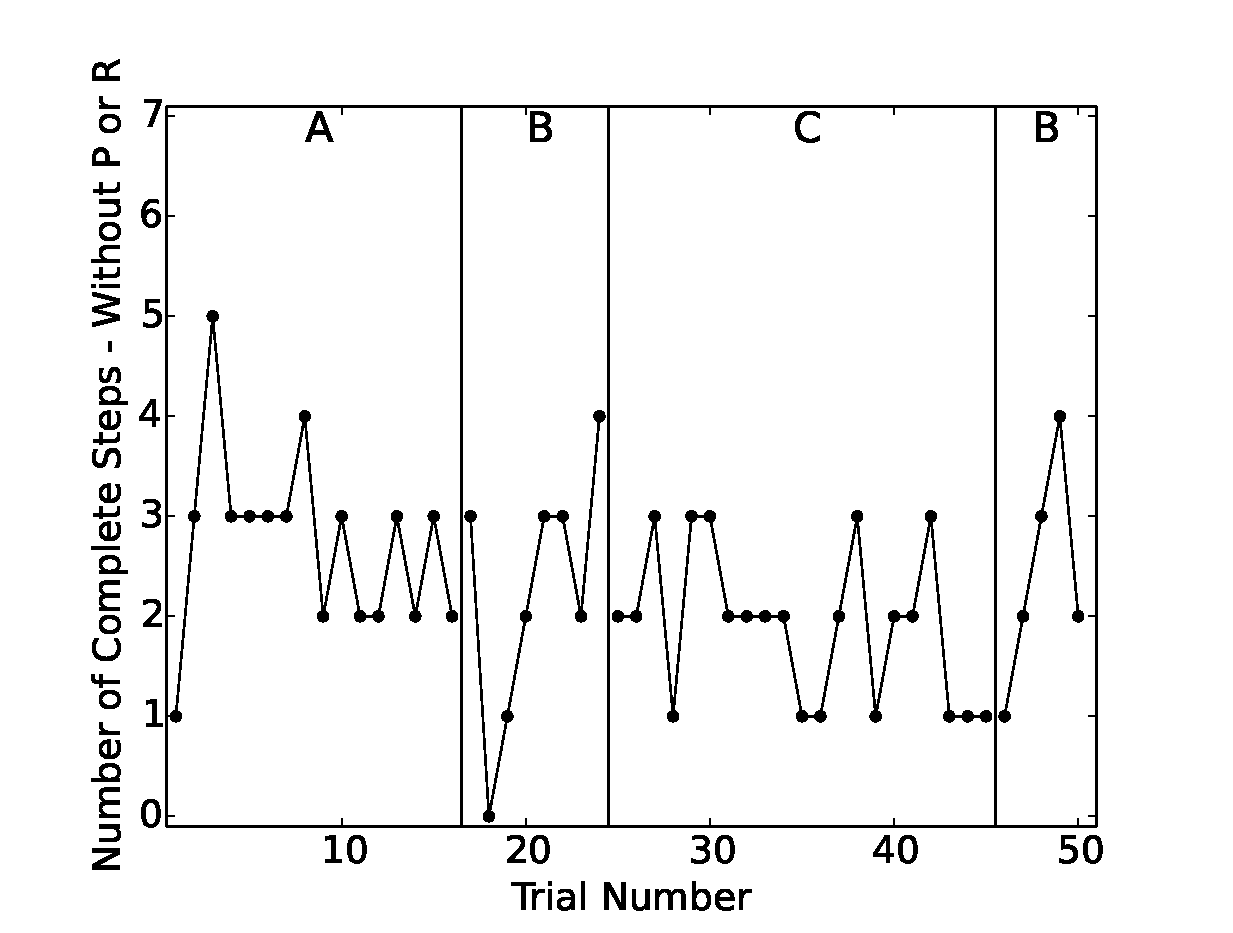
\includegraphics[width=1.1\linewidth]{./img/data_analysis/110NumberofCompleteSteps-WithoutPorR.eps}
		\caption{Total Number of Complete Steps - Without Prompts}
		\label{fig:7TotalNumberofCompleteSteps-WithoutPrompts}
	\end{subfigure}
	\hfill
	%	~ %add desired spacing between images, e. g. ~, \quad, \qquad, \hfill, or double enter etc.	
	\begin{subfigure}[b]{0.49\textwidth}
		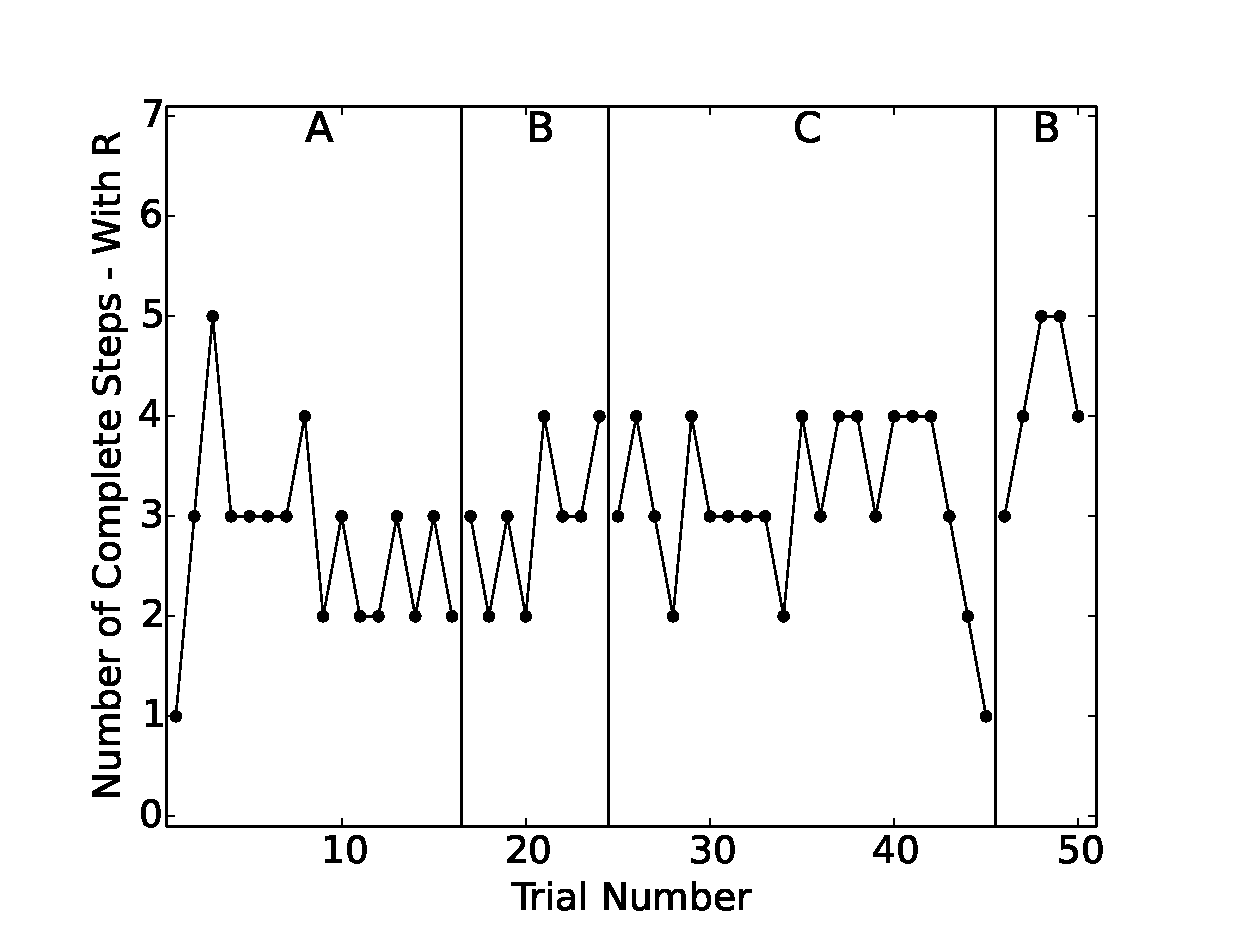
\includegraphics[width=1.1\linewidth]{./img/data_analysis/109NumberofCompleteSteps-WithR.eps}
		\caption{Total Number of Complete Steps - With Robot Prompts Only}
		\label{fig:6TotalNumberofCompleteSteps-WithRobotPrompts}
	\end{subfigure}%
	
	
	\begin{subfigure}[b]{0.49\textwidth}
		
\includegraphics[width=1.1\linewidth]{./img/data_analysis/blank.png}
	\end{subfigure}%
	\hfill
	\begin{subfigure}[b]{0.49\textwidth}
		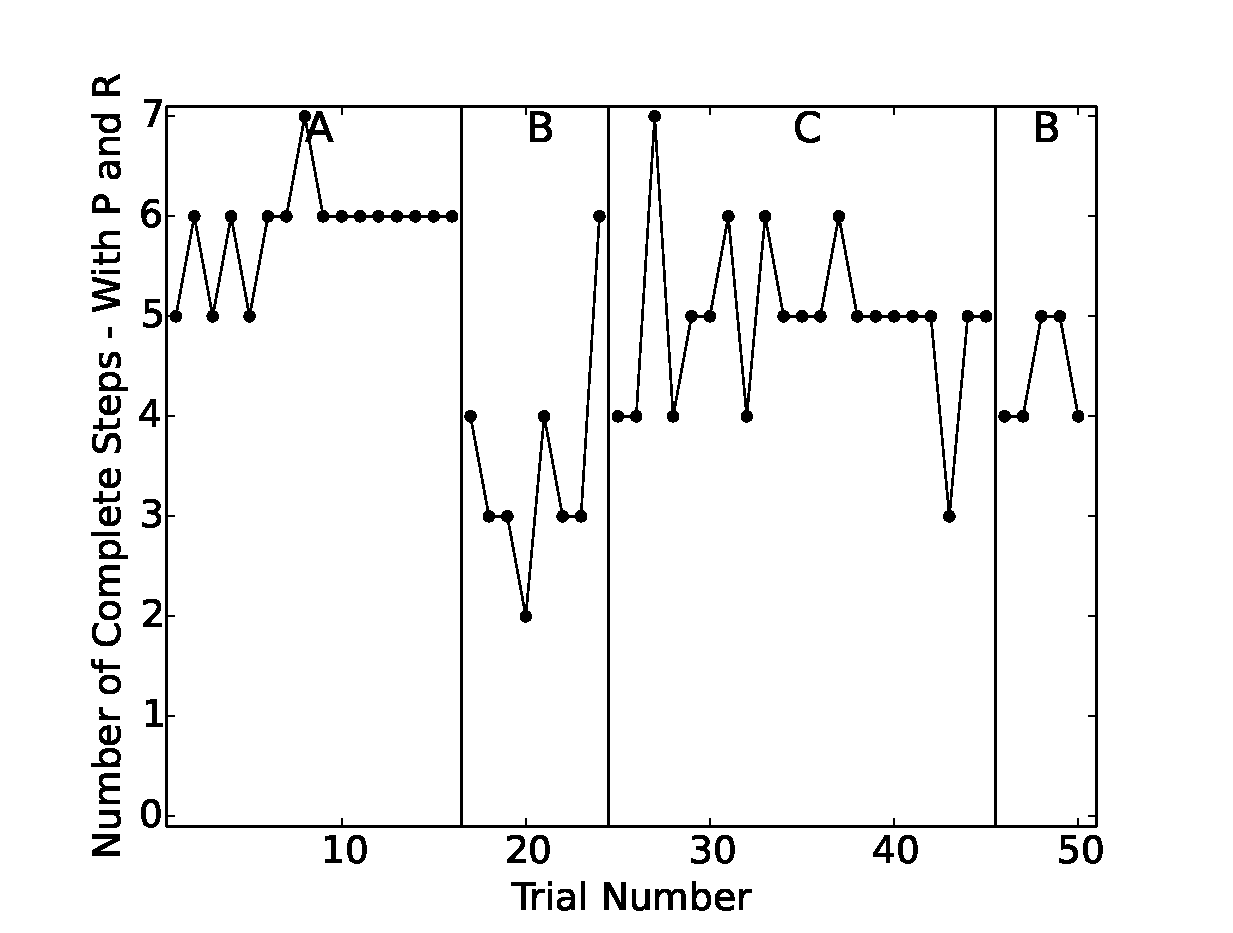
\includegraphics[width=1.1\linewidth]{./img/data_analysis/108NumberofCompleteSteps-WithPandR.eps}
		\caption{Total Number of Complete Steps - With Robot and Parent Prompts}
		\label{fig:4TotalNumberofCompleteSteps-WithRobotAndParentPrompts}
	\end{subfigure}%
	\caption{Total Number of Complete Steps}
	\label{fig:TotalNumberOfIncompleteSteps}
\end{figure}

\paragraph{Number of Parent Prompts}
The measure ``Total Number of Parent Prompts'' is plotted in Figure \ref{fig:TotalNumberOfParentPrompts}.  Plot \ref{fig:25TotalNumberofParentPrompts} is for the overall count (i.e. counting both physical and non-physical prompts).  It shows that during parent alone phase (A), the measure has an upward trend from 5 moving to 20.  However, in robot alone phase (first Phase B), we have a sudden drop leveling at near zero.  In robot parent phase (C), the measure has a downward trend moving from 15 to 5.  In robot alone repeat phase (second Phase B), we again observe a near zero level.  By comparing the measures across phases, we see that the robot's presence were effective in reducing the number of parent prompts, especially in robot alone and repeat phases.  Plot \ref{fig:26TotalNumberofParentPrompts-Physical} is for the physical prompt count.  This plot shows when the parent resorts to a higher prompt level (i.e. physical prompts such as nudging, guiding, and physically intervene) in order to get the child's compliance.  We see that the level is mainly near zero for all phases except for robot parent phase (C), leveling around 2.5.
\begin{figure}[h]
	\centering
	\begin{subfigure}[b]{0.49\textwidth}
		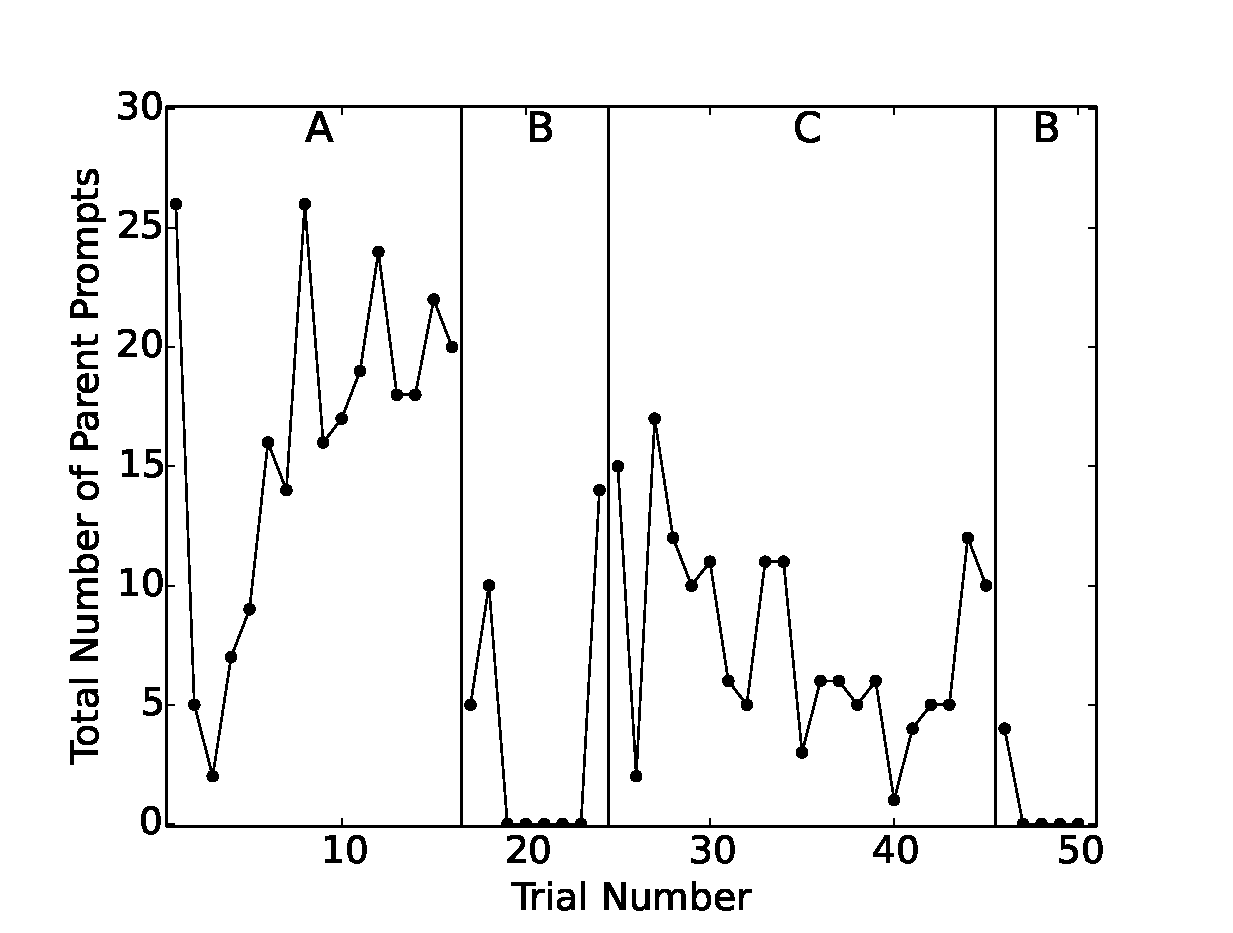
\includegraphics[width=1.1\linewidth]{./img/data_analysis/25TotalNumberofParentPrompts.eps}
		\caption{Total Number of Parent Prompts - Overall}
		\label{fig:25TotalNumberofParentPrompts}
	\end{subfigure}
	\hfill
	\begin{subfigure}[b]{0.49\textwidth}
		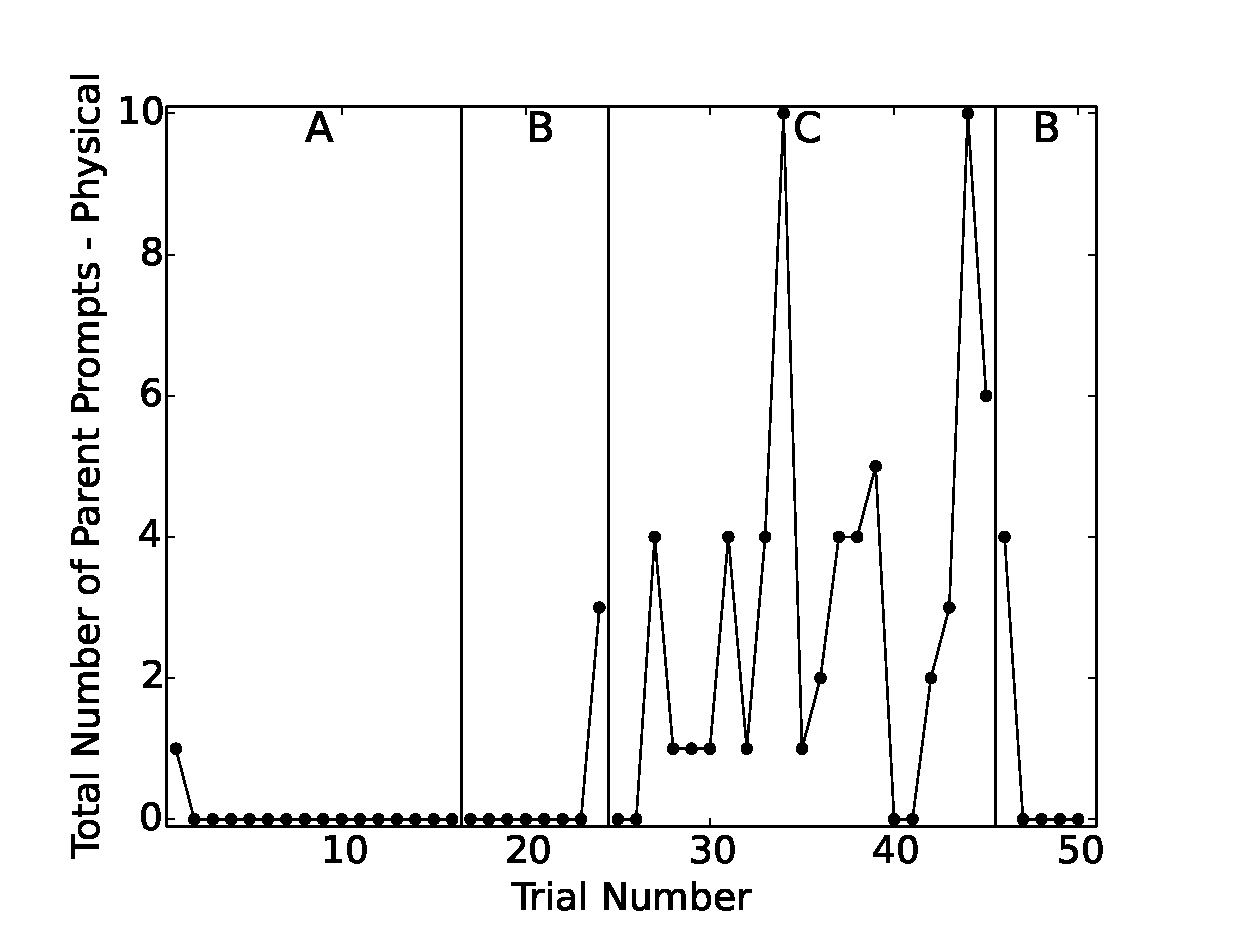
\includegraphics[width=1.1\linewidth]{./img/data_analysis/26TotalNumberofParentPrompts-Physical.eps}
		\caption{Total Number of Parent Prompts - Physical}
		\label{fig:26TotalNumberofParentPrompts-Physical}
	\end{subfigure}%
	\caption{Total Number of Parent Prompts}
	\label{fig:TotalNumberOfParentPrompts}
\end{figure}


\subsubsection{Child's Response to Prompts}
To illustrate the child's different responses to the prompts, we characterized child's responses into three categories: ``compliance'', ``not affected by prompt'', and others.

\paragraph{Compliance Rate}
A response is counted towards ``compliance'' if the child executes the correct step in response to the prompt.  If the child was executing the wrong step before prompt, and is converted into doing the correct step due to prompt, we call this hard compliance.  The compliance and hard compliance response rates are shown in Figure \ref{fig:ComplianceRate}.

Plot \ref{fig:102ComplianceRate-Overall} shows the overall compliance rate, with parent alone phase (A) leveling at 80\%, robot alone phase (first Phase B) leveling at 30\%, parent robot phase (C) moving upward from 60\% to 80\%, and robot alone repeat phase (second Phase B) leveling at 80\%.  We see that when the robot was first introduced in robot alone phase (first Phase B), the child did not comply to the prompts.  However, by going through Phase C where the parent prompts for the child to follow the robot, the child complies more readily in the robot alone repeat phase, achieving similar level of compliance as the parent alone phase.  We need to note that this plot includes prompts delivered by the robot, by the parent, and by them together.  Even in robot alone and repeat phases, the parent still comes into the washroom and prompts when the child isn't complying to the robot.  To see whether the robot alone can potentially guide the child through the whole hand-washing activity with minimal parent involvement, we plotted the compliance rate counted over only prompts delivered by the robot, shown in Plot \ref{fig:79ComplianceRate-R1Pv0g0}.  This plot confirms the levels observed in the overall plot, validating the improvement of compliance rate seen in R Alone Rep phase.  To investigate to what extent the child is compliant, the overall hard compliance rate is shown in Plot \ref{fig:103HardComplianceRate-Overall}, with parent alone phase (A) split leveling at 100\% and 35\%, robot alone phase (first Phase B) leveling at 25\%.  The robot parent phase (C) averaging around 60\% but the spread increases as trials went on.  Lastly, the robot alone repeat phase (second Phase B) levels at 50\%.  Similar to above, we observe an improvement of hard compliance between robot alone and repeat phases.  Looking at the robot prompts only Plot \ref{fig:92HardComplianceRate-R1Pv0g0}, the robot alone phase (first Phase B) drops to almost 0\%, while robot alone repeat phase (second Phase B) remains at 50\%.
\begin{figure}[h]
	\centering
	\begin{subfigure}[b]{0.49\textwidth}
		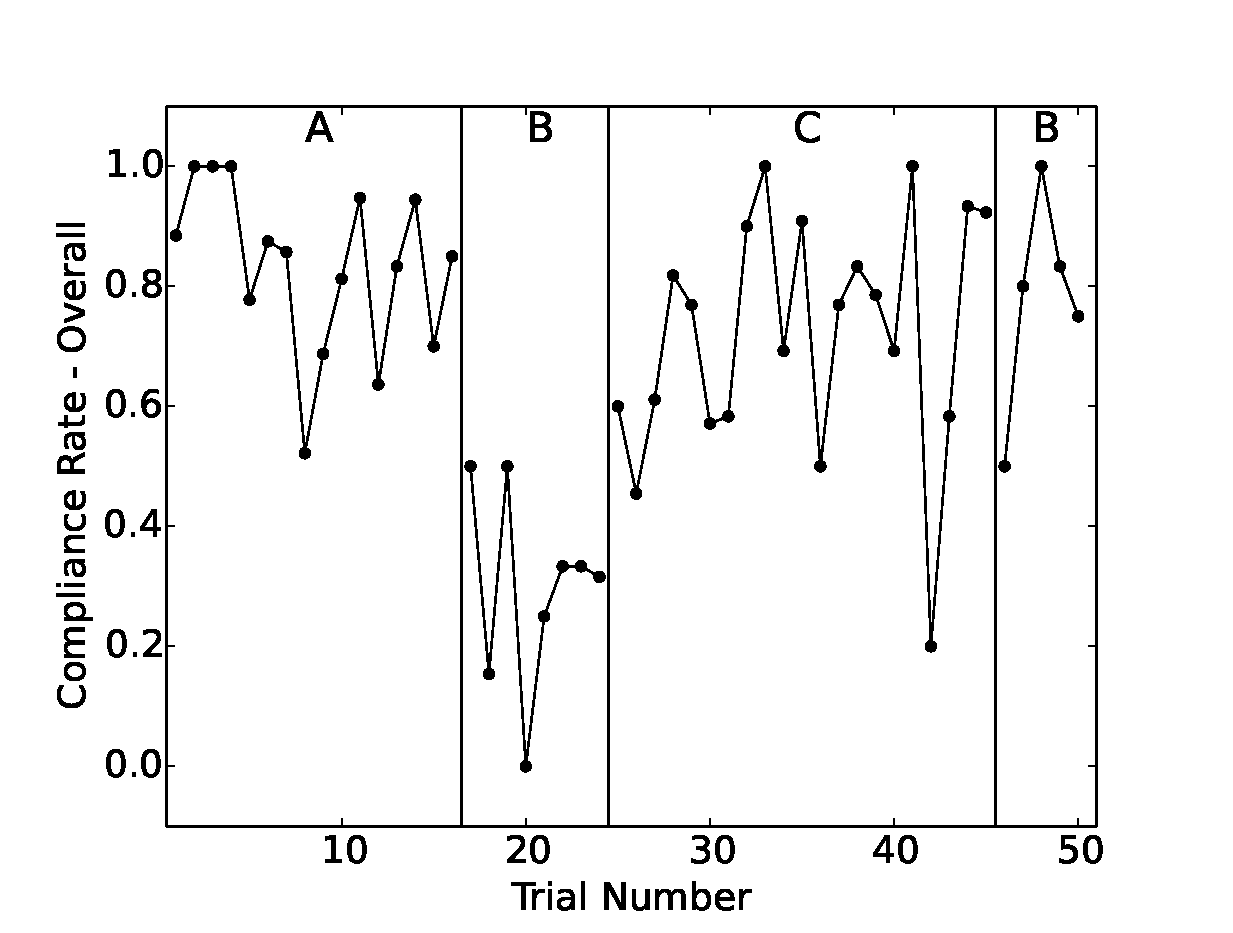
\includegraphics[width=1.1\linewidth]{./img/data_analysis/102ComplianceRate-Overall.eps}
		\caption{Compliance Rate - Overall}
		\label{fig:102ComplianceRate-Overall}
	\end{subfigure}
	\hfill
	\begin{subfigure}[b]{0.49\textwidth}
		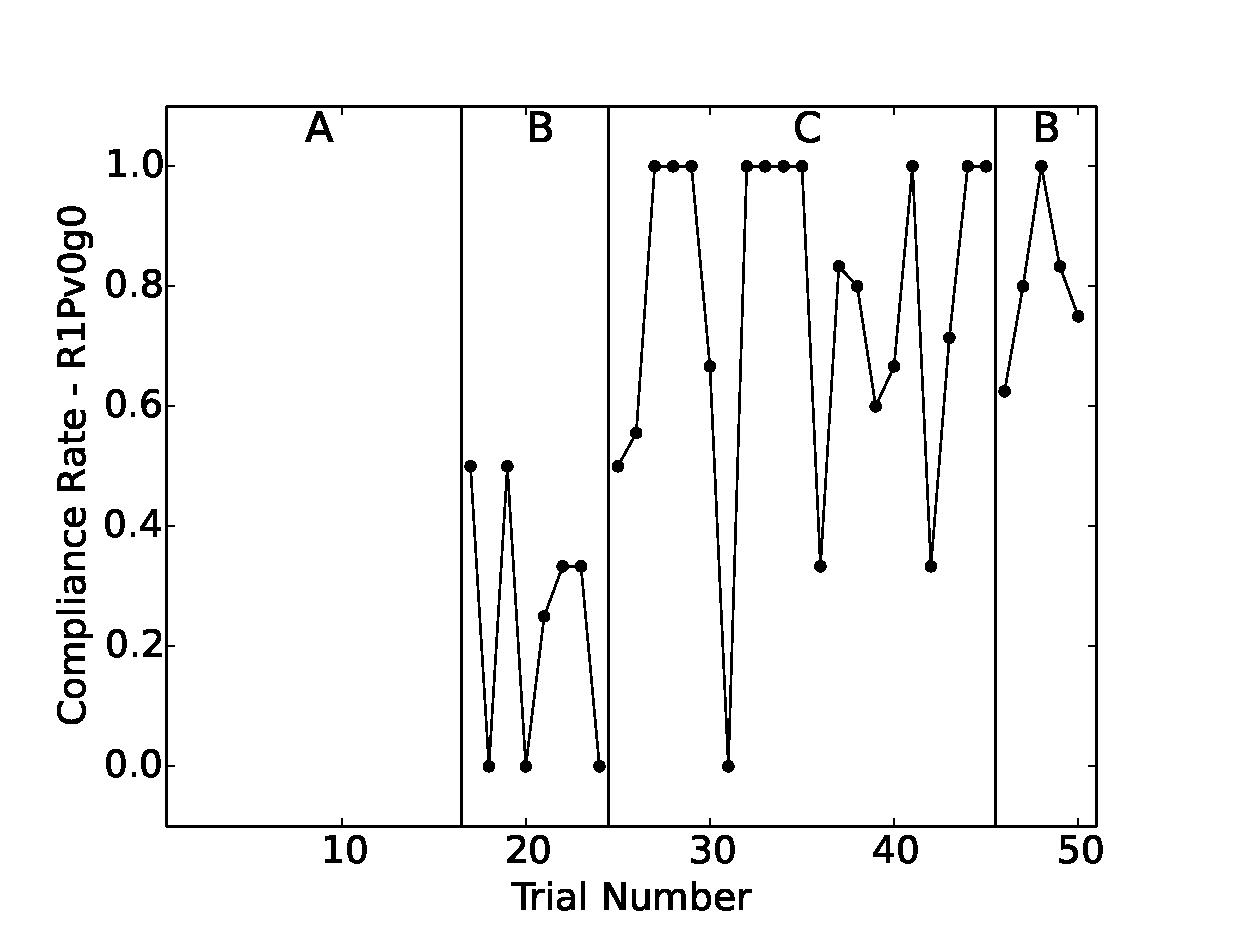
\includegraphics[width=1.1\linewidth]{./img/data_analysis/79ComplianceRate-R1Pv0g0.eps}
		\caption{Compliance Rate - Robot Only Prompts}
		\label{fig:79ComplianceRate-R1Pv0g0}
	\end{subfigure}%
	
	
	\begin{subfigure}[b]{0.49\textwidth}
		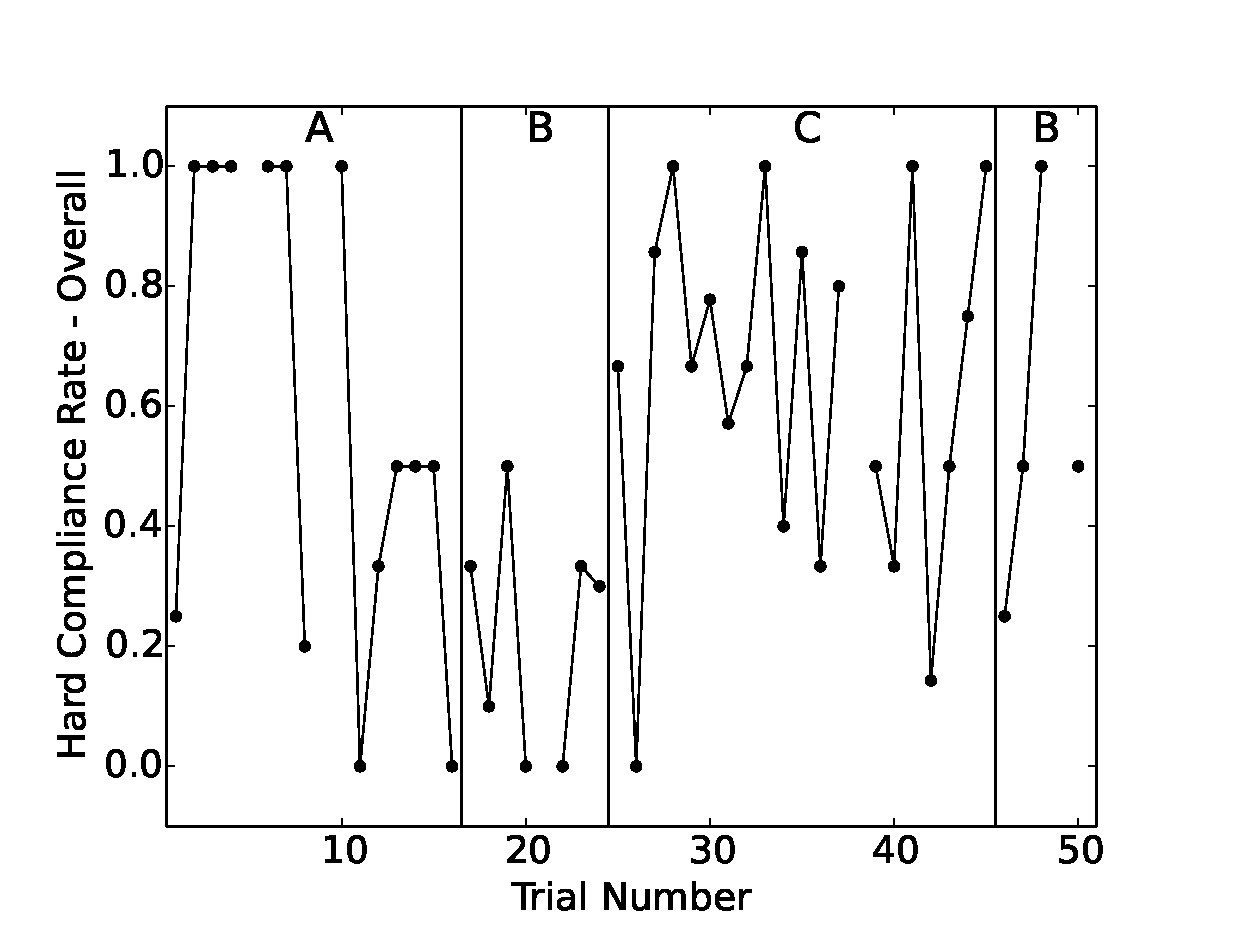
\includegraphics[width=1.1\linewidth]{./img/data_analysis/103HardComplianceRate-Overall.eps}
		\caption{Hard Compliance Rate - Overall}
		\label{fig:103HardComplianceRate-Overall}
	\end{subfigure}
	\hfill
	\begin{subfigure}[b]{0.49\textwidth}
		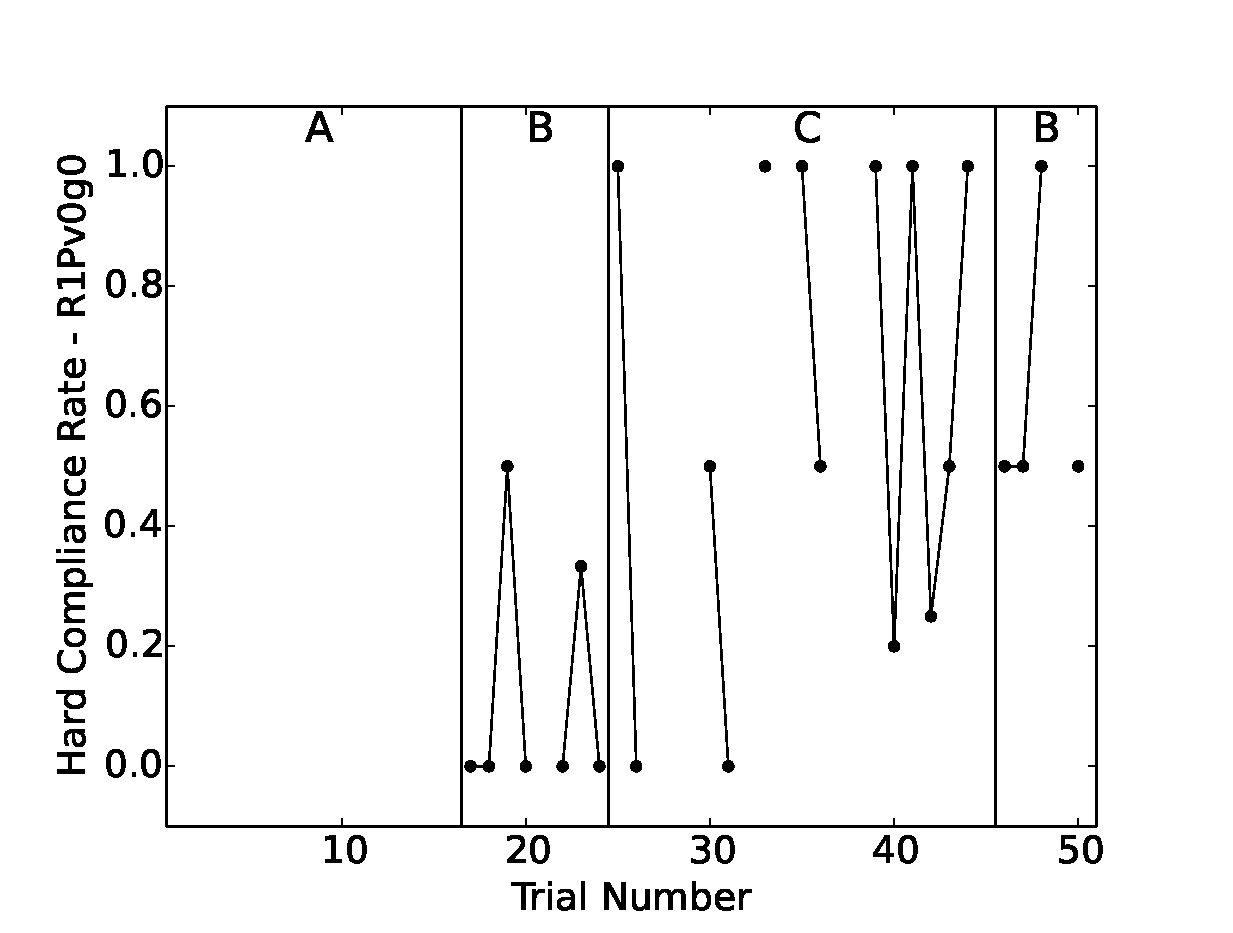
\includegraphics[width=1.1\linewidth]{./img/data_analysis/92HardComplianceRate-R1Pv0g0.eps}
		\caption{Hard Compliance Rate - Robot Only Prompts}
		\label{fig:92HardComplianceRate-R1Pv0g0}
	\end{subfigure}%
	\caption{Compliance Rate}
	\label{fig:ComplianceRate}
\end{figure}

\paragraph{Not Affected By Prompt Rate}
A response is counted towards ``not affected by prompt'' if the child was executing a wrong step and did not change after the prompt or was idling and did not change after the prompt.  The not affected by prompt rate is shown in Plot \ \ref{fig:99NotAffectedByPromptRate-Overall}.  We see that for most phases, it levels at 15\%, but for robot alone repeat phase (second Phase B) it is at 35\%.  This shows the robot prompts were ignored more when the robot was first introduced, but improves to an acceptable level through Phase C.
\begin{figure} [h]
	\centering
	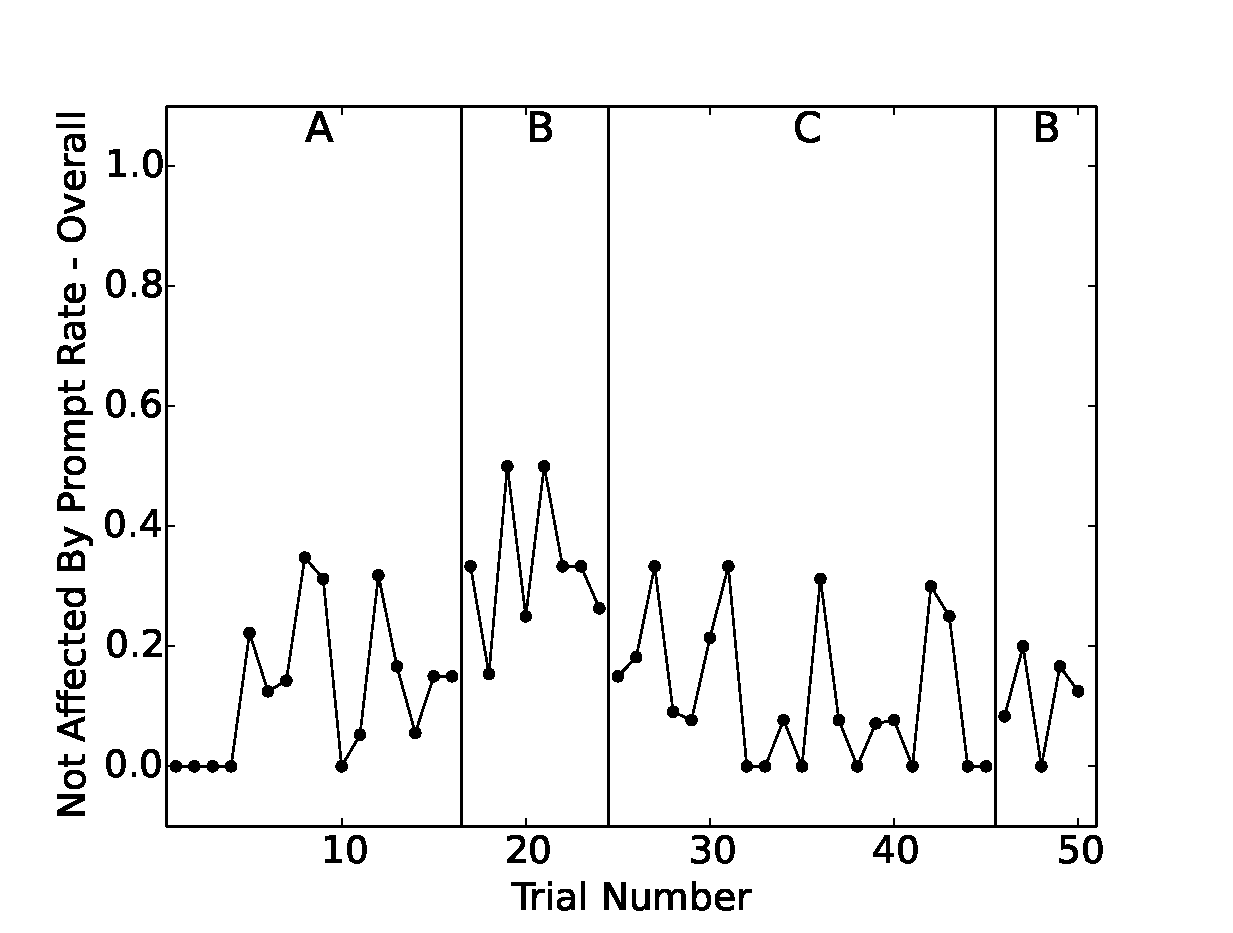
\includegraphics[width=0.6\textwidth]{./img/data_analysis/99NotAffectedByPromptRate-Overall.eps}
	\caption{Not Affected By Prompt Rate}
	\label{fig:99NotAffectedByPromptRate-Overall}
\end{figure}


\subsubsection{Engagement and Visual Attention}
To further characterize child's response to different prompting phases, we investigate how many times the child smiles and murmurs during step execution, and how often the child looks at the prompting agent during prompting and step execution.

\paragraph{Number of Times Child Smiles}
The measure ``Total Number of Times Child Smiles'' is shown in Plot \ \ref{fig:12TotalNumberofTimesChildSmiles}.  In it, parent alone phase (A) levels at 1.5, robot alone phase (first Phase B) levels at 0.5, robot parent phase (C) has a large spread and averages around 3, and robot alone repeat phase (second Phase B) also has a large spread and averages around 4.  It shows that the child smiles much more in later phases compared to earlier phases, and particularly, smiles in the repeat phase more than in robot alone phase.
\begin{figure} [h]
	\centering
	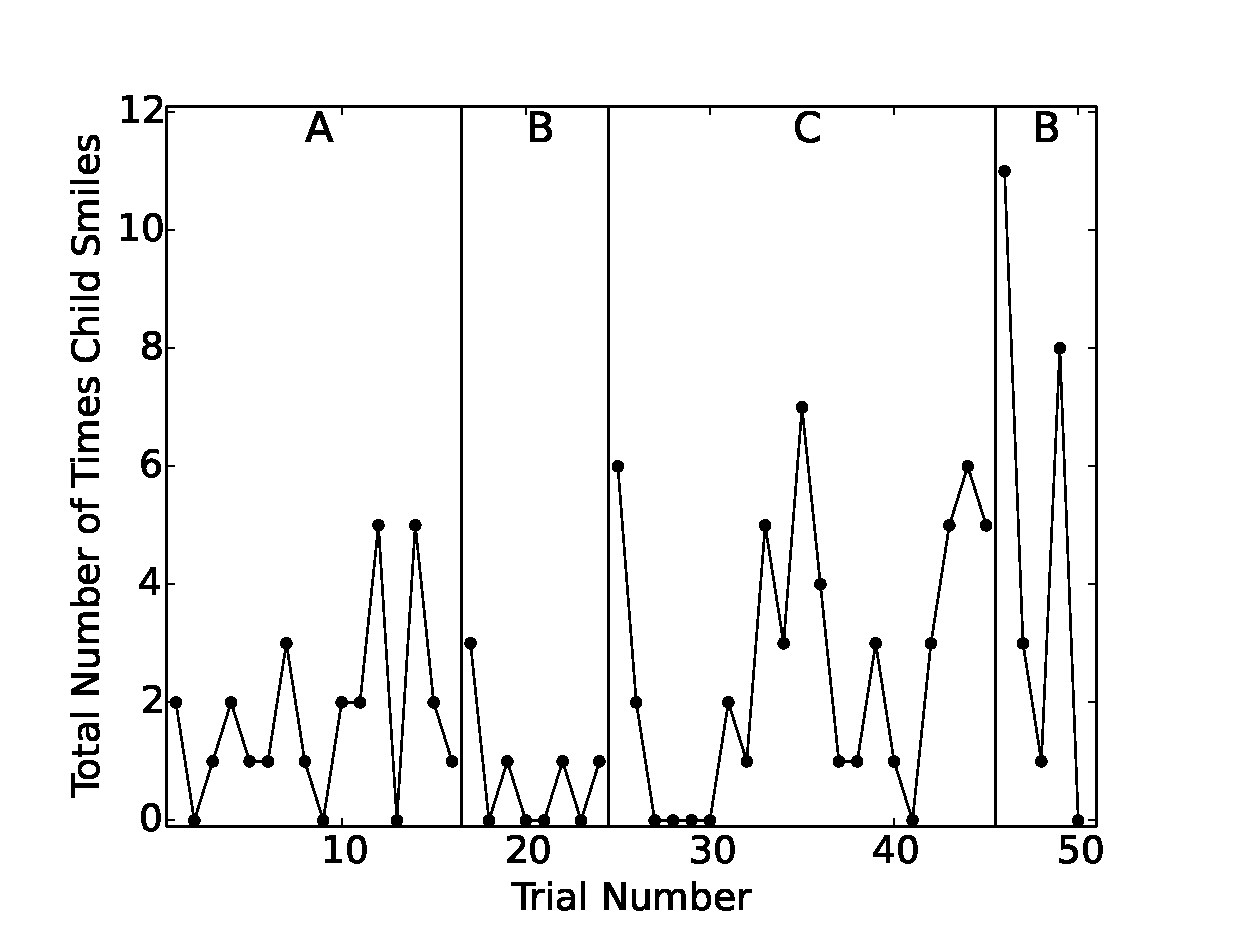
\includegraphics[width=0.6\textwidth]{./img/data_analysis/12TotalNumberofTimesChildSmiles.eps}
	\caption{Total Number of Times Child Smiles}
	\label{fig:12TotalNumberofTimesChildSmiles}
\end{figure}



\paragraph{Number of Times Child Murmurs}
The measure ``Total Number of Times Child Murmurs'' is shown in Plot \ \ref{fig:13TotalNumberofTimesChildMurmurs}.  In it, parent alone phase (A) has a large spread, averaging around 4.  Robot alone phase (first Phase B) levels at 0.5.  Robot parent phase (C) has a large spread, averaging around 4.  Robot alone repeat phase (second Phase B) levels at 2.  It shows that the child murmurs much more often when the parent is present.  Also, child murmurs in the repeat phase more than the robot alone phase.
\begin{figure} [h]
	\centering
	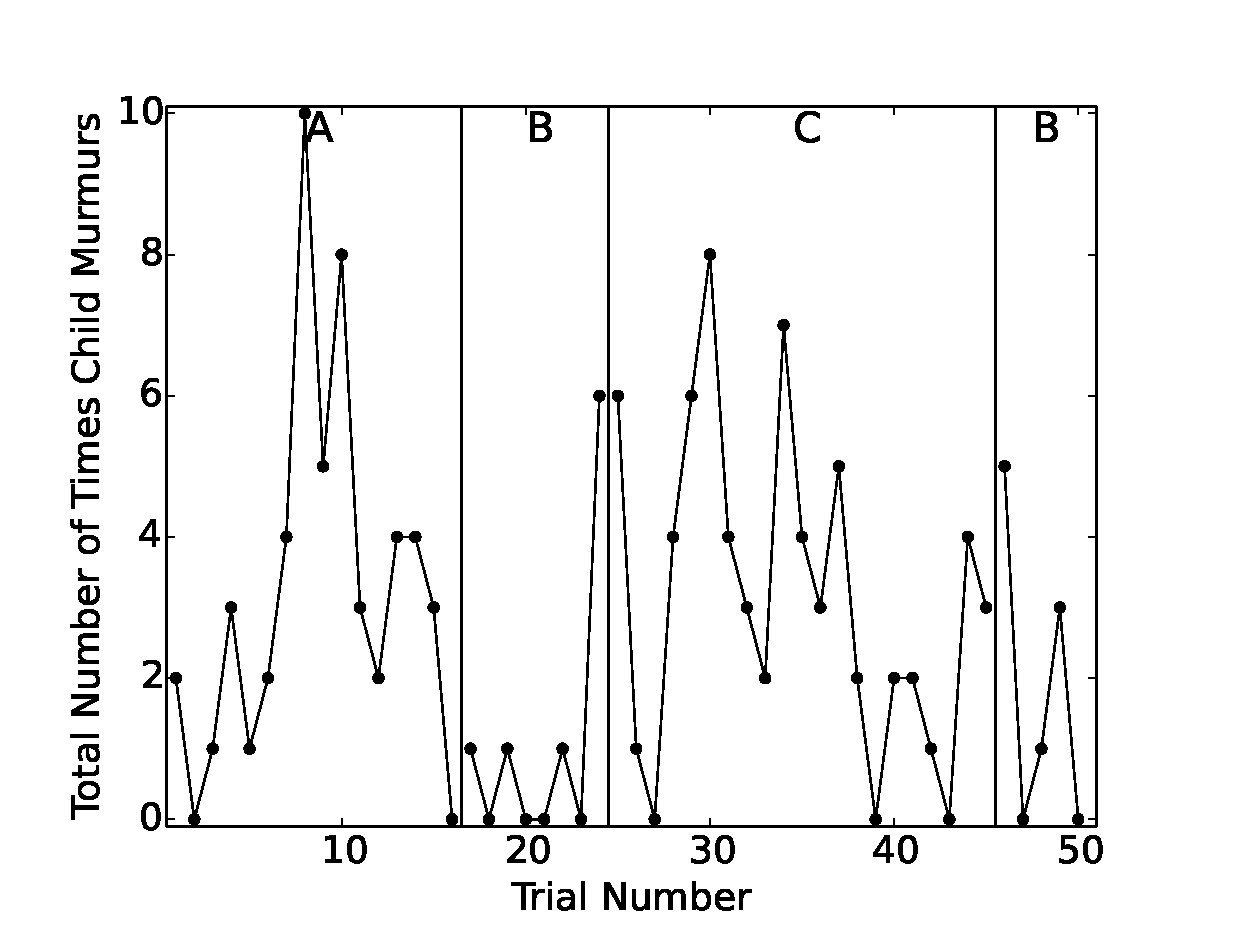
\includegraphics[width=0.6\textwidth]{./img/data_analysis/13TotalNumberofTimesChildMurmurs.eps}
	\caption{Total Number of Times Child Murmurs}
	\label{fig:13TotalNumberofTimesChildMurmurs}
\end{figure}

\paragraph{Looking at Prompting Agent Rate}
A prompt can be given by the parent, by the robot, or by them together.  During prompting and during step execution, the child may turn and look at the parent and/or the robot.  The gaze behavior of the child is shown in Figure \ref{fig:LookingAtPromptingAgentDuringPrompts} for all the cases above.  Because not all cases have the same amount of data in all phases, we will only mention here the phases that have enough evidence.  In Plot \ref{fig:8LookingatParentRateGivenParentPrompted}, ``Looking at Parent Rate - Given Parent Prompted'' levels at 40\% in parent alone phase (A).  In Plot \ref{fig:92HardComplianceRate-R1Pv0g0}, ``Looking at Robot Rate - Given Robot Prompted'' trends downward from 50\% to 30\% for robot alone phase (first Phase B), levels at 30\% with high spread for robot parent phase (C), and levels at 20\% for robot alone repeat phase (second Phase B).  We see that when the parent and the robot prompt individually, the parent has a higher chance of getting the child's visual attention.  Although the robot had similar levels of attention when was first introduced, it dropped as the study went on.  In Plot \ref{fig:10LookingatParentRateGivenBothPrompted}, ``Looking at Parent Rate - Given Both Prompted'' averages around 50\% with high spread in robot parent phase (C).  In Plot \ref{fig:11LookingatRobotRateGivenBothPrompted}, ``Looking at Robot Rate - Given Both Prompted' levels at 15\% for robot parent phase (C).  We see that when the parent and the robot prompt at the same time, the parent had a greater amount of visual attention.  It is interesting to note that the parent had similar levels of visual attention when prompting alone and when prompting with the robot.  The robot, however, experienced a decrease in visual attention level when the parent prompts with it.
\begin{figure}[h]
	\centering
	\begin{subfigure}[b]{0.49\textwidth}
		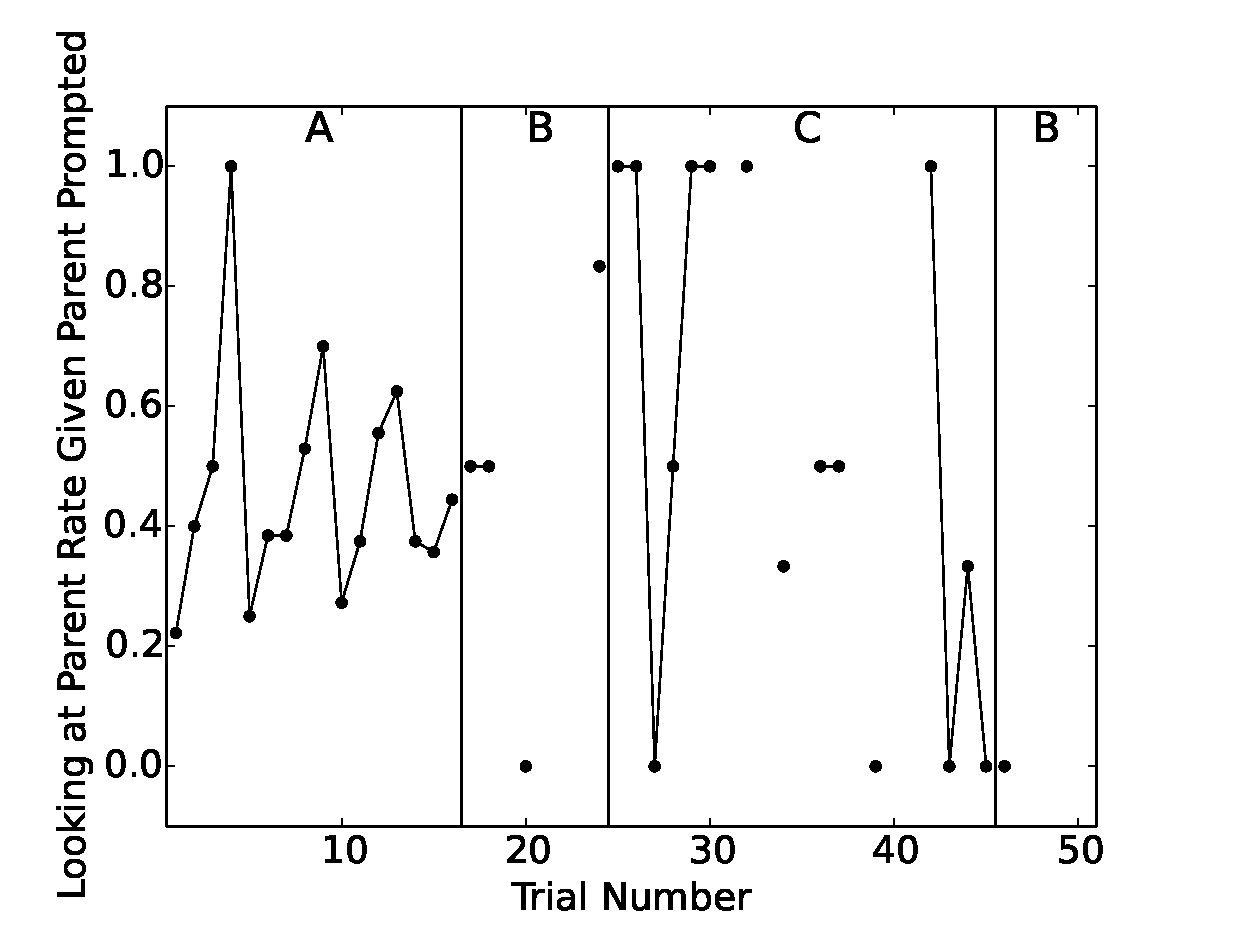
\includegraphics[width=1.1\linewidth]{./img/data_analysis/8LookingatParentRateGivenParentPrompted.eps}
		\caption{Looking at Parent Rate - Given Parent Prompted}
		\label{fig:8LookingatParentRateGivenParentPrompted}
	\end{subfigure}
	\hfill
	\begin{subfigure}[b]{0.49\textwidth}
		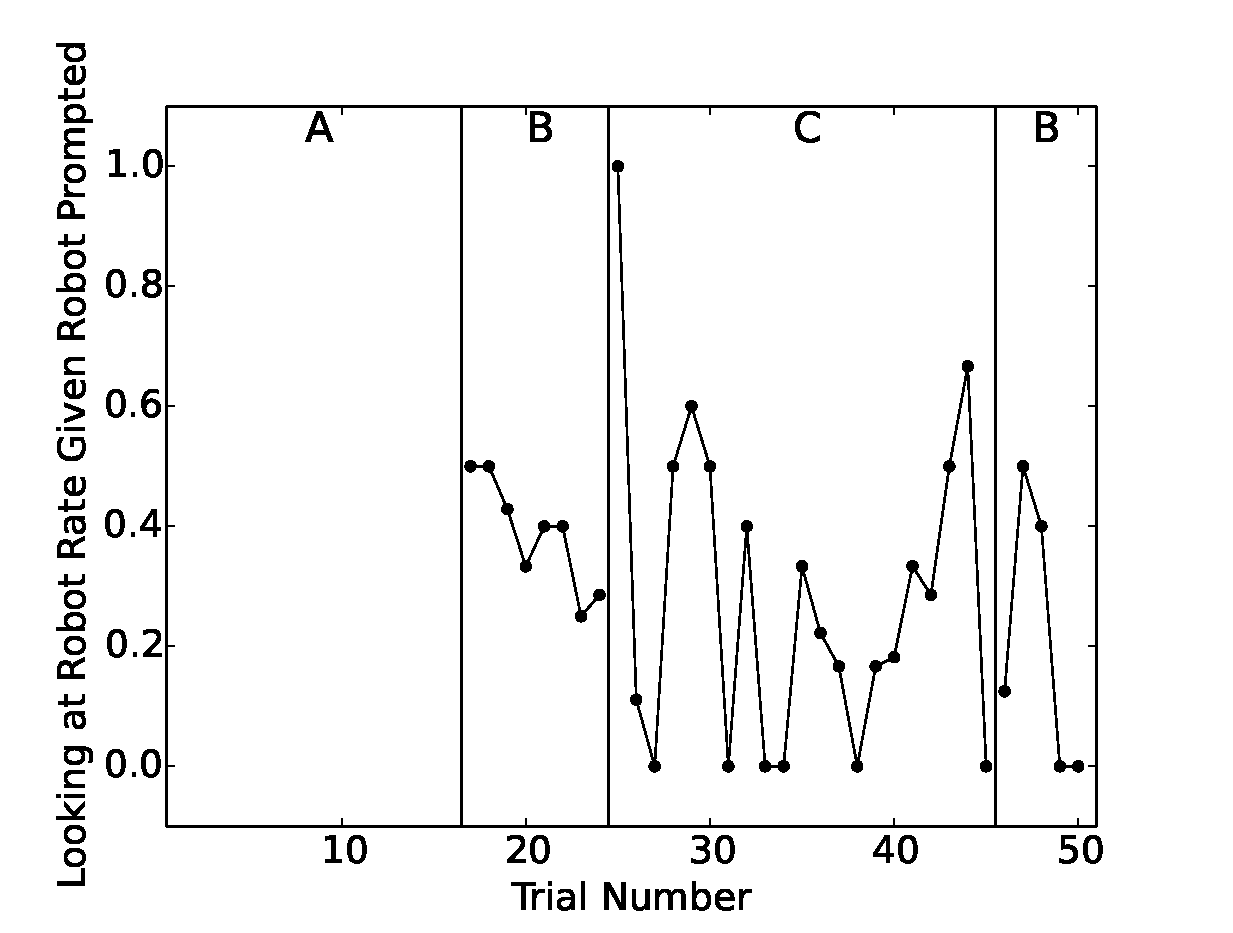
\includegraphics[width=1.1\linewidth]{./img/data_analysis/9LookingatRobotRateGivenRobotPrompted.eps}
		\caption{Looking at Robot Rate - Given Robot Prompted}
		\label{fig:9LookingatRobotRateGivenRobotPrompted}
	\end{subfigure}%
	
	
	\begin{subfigure}[b]{0.49\textwidth}
		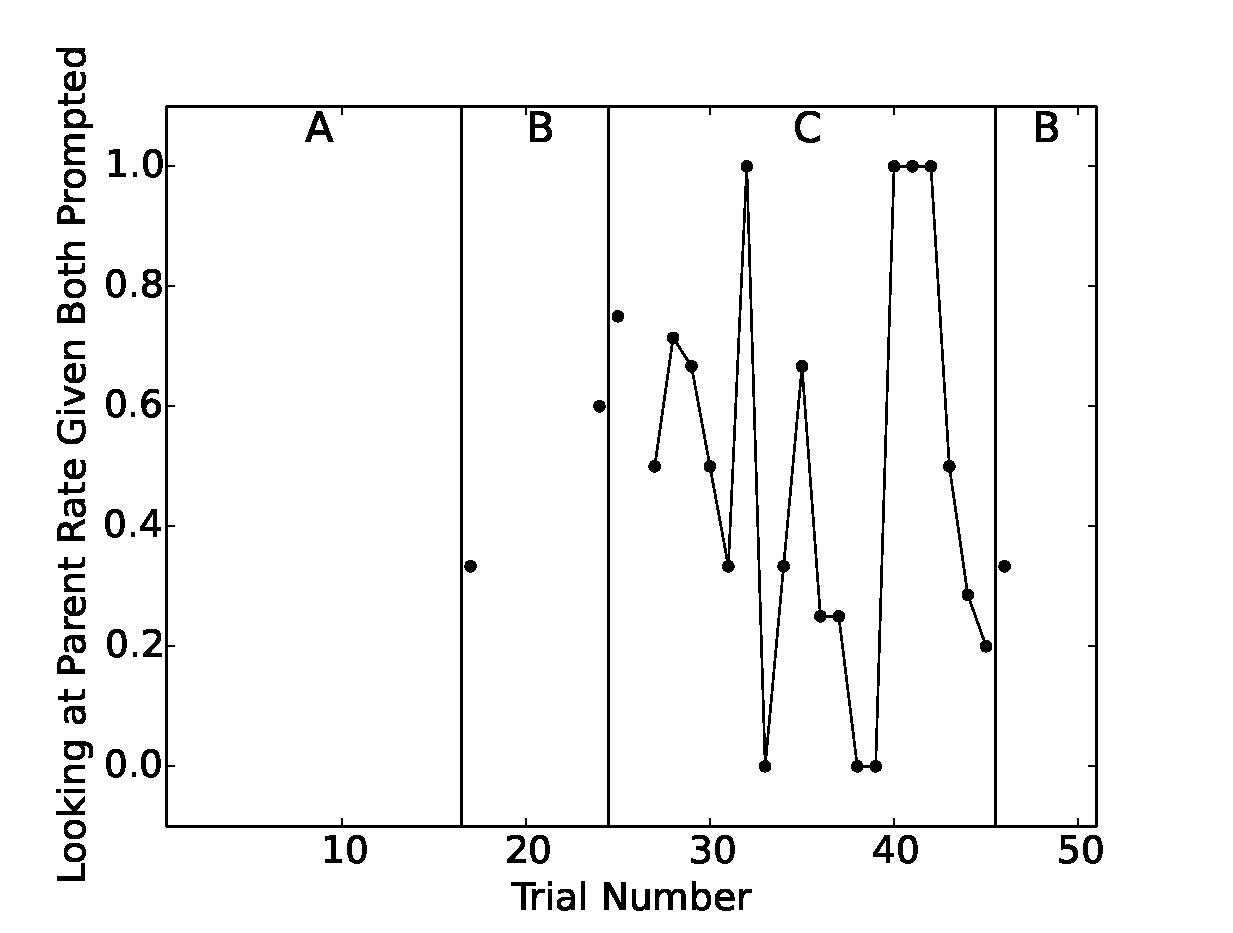
\includegraphics[width=1.1\linewidth]{./img/data_analysis/10LookingatParentRateGivenBothPrompted.eps}
		\caption{Looking at Parent Rate - Given Both Prompted}
		\label{fig:10LookingatParentRateGivenBothPrompted}
	\end{subfigure}
	\hfill
	\begin{subfigure}[b]{0.49\textwidth}
		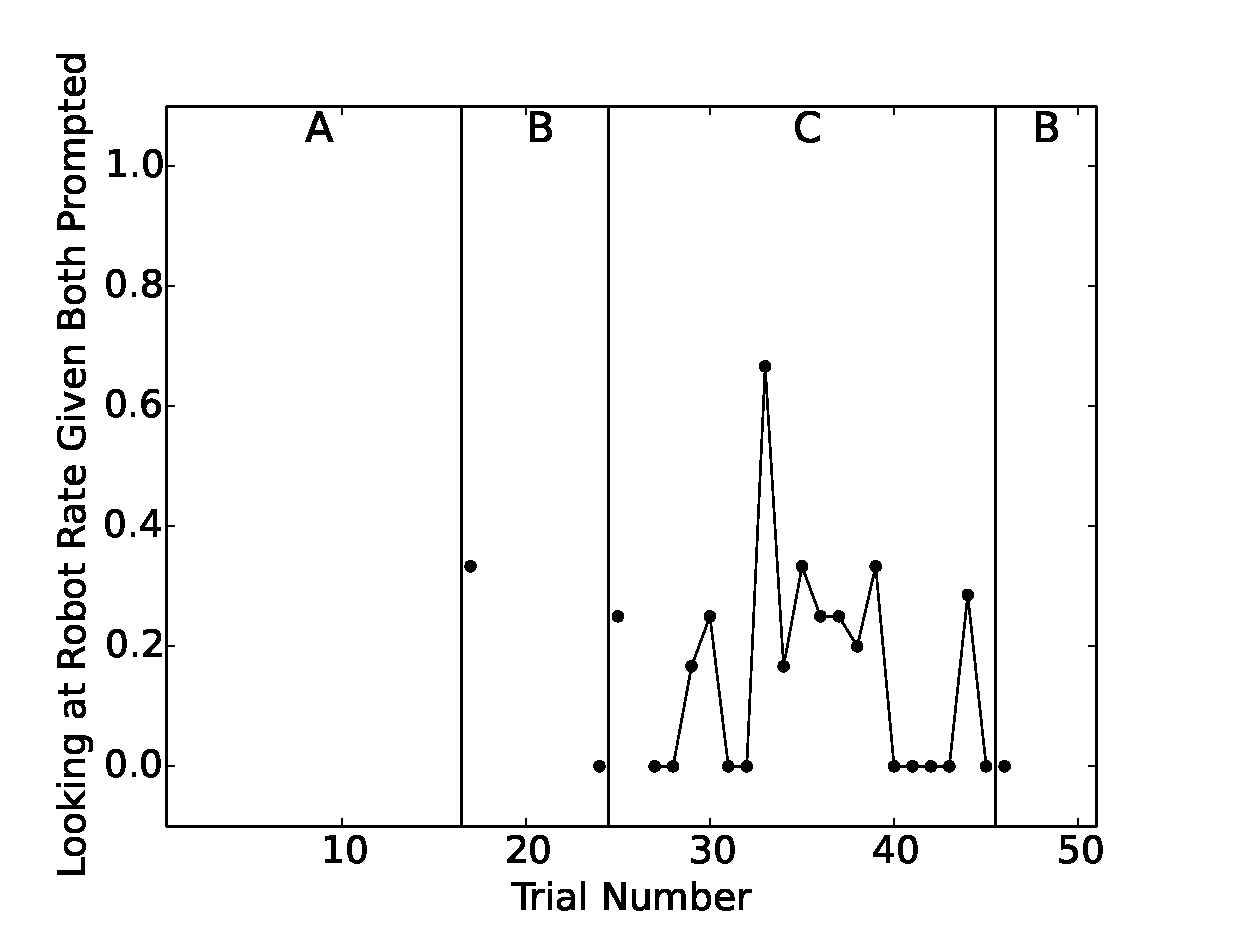
\includegraphics[width=1.1\linewidth]{./img/data_analysis/11LookingatRobotRateGivenBothPrompted.eps}
		\caption{Looking at Robot Rate - Given Both Prompted}
		\label{fig:11LookingatRobotRateGivenBothPrompted}
	\end{subfigure}%
	\caption{Looking at Prompting Agent Rate}
	\label{fig:LookingAtPromptingAgentDuringPrompts}
\end{figure}
